%% LyX 2.3.3 created this file.  For more info, see http://www.lyx.org/.
%% Do not edit unless you really know what you are doing.
\documentclass[english]{article}
\usepackage[T1]{fontenc}
\usepackage[latin9]{inputenc}
\usepackage{babel}
\usepackage{float}
\usepackage{wrapfig}
\usepackage{amssymb}
\usepackage{graphicx}
\usepackage[unicode=true]
 {hyperref}

\makeatletter
%%%%%%%%%%%%%%%%%%%%%%%%%%%%%% User specified LaTeX commands.
\usepackage{algorithm,algpseudocode}

\makeatother

\usepackage[style=numeric]{biblatex}
\addbibresource{project.bib}
\begin{document}
\title{CS221 project proposal: Motion Planning for Autonomous Driving}
\author{Philippe Weingertner, Minnie Ho}
\maketitle

\section{Problem definition}

We study the motion planning problem for Autonomous Driving. The behavioral
planner defines a short term objective: where the ego vehicle shall
go, with associated constraints. The local planner then computes a
set of paths that are kinematically feasible and collision free with
respect to static obstacles. For every candidate path, a velocity
profile is generated to avoid dynamic obstacles. This two steps decomposition
of local planning is typical to make the problem simpler to solve
in real time.

\begin{wrapfigure}{R}{0.2\columnwidth}%
\begin{raggedleft}
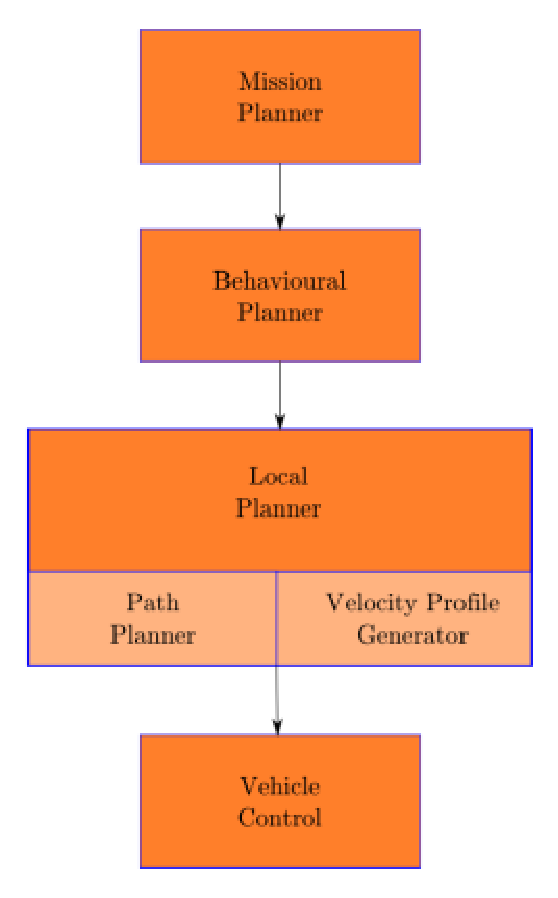
\includegraphics[scale=0.18]{img/dpl}
\par\end{raggedleft}
\end{wrapfigure}%

Given a path to follow and information about dynamic obstacles, we
have to define a velocity profile such that the trajectory is collision
free, comfortable (without too strong accelerations or decelerations)
and efficient (as close as possible to the target velocity). An autonomous
vehicle has to deal with many sources of uncertainties. We consider
sensor uncertainty and driving model uncertainty which translate to
dynamics uncertainties. On the social impact aspect, as mentionned
in \cite{article}: ``Autonomous vehicles are one of the most highly
anticipated technological developments of our time, with potentially
wide-ranging social implications''.

\section{Proposed Approach}

To define our Oracle we consider there is no uncertainty: sensors
are perfect and we know the driving models of every car. The Oracle
is a search algorithm without real-time constraints. To define our
baseline we set a simple rule for decision making: if the smallest
Time To Collision with respect to other cars is below 10 seconds we
decelerate by $-2m.s^{-2}$ (as long as we see this collision risk)
otherwise we accelerate at $1m.s^{-2}$ (as long as we are below the
speed limit) to reach our target as fast as possible.

Ultimately we will handle this problem as a MDP search problem as
we are dealing with uncertainty and we want to investigate how we
can improve real-time performances. One possible track, as in \cite{DBLP:journals/corr/abs-1905-02680},
is to combine planning and learning \cite{DBLP:journals/corr/abs-1803-10056},
in a similar way to AlphaZero \cite{DBLP:journals/corr/abs-1712-01815},
to have a good heuristic to efficiently guide the search of a MCTS
tree search \cite{Kochenderfer2015} used for solving online our MDP
problem.

\subsection{Model}

The state space is continuous whereas the action space is discrete.
The model used by our Oracle is the following:
\begin{itemize}
\item \textbf{startState}: random initialization with 5 cars on the left
and 5 cars on the right with trajectories crossing the middle path,
of the ego vehicle. All the speed are initialized around $20ms^{-1}.$
The ego vehicle is $200m$ away from its target point: it shall find
a velocity profile that is efficient (fast), comfortable (limiting
strong decelerations and accelerations) and collision free for the
proposed path.
\item \textbf{isEnd}: when target is reached by the ego vehicle
\item \textbf{states}: a vector in $\mathbb{R}^{44}$ with $[x,y,\dot{x},\dot{y}]$
for 10+1 objects
\item \textbf{actions}: every $250$ ms we choose an acceleration command
out of  $\{-2,-1,0,1,2\}\;m.s^{-2}$ 
\item \textbf{succAndCost}: the new state is computed based on a Constant
Acceleration (over a time step) model for the cars. The cost is $1000$
for a collision, 1 for an acceleration command $\in[-1,0,1]\;ms^{-2}$
and 2 for uncomfortable accelerations $\pm2\;ms^{-2}$. The evolution
from one state to the next state is deterministic: with probability
1 the surrounding vehicles use an acceleration of $0.$ We will introduce
uncertainty later on. 
\end{itemize}

\subsection{Algorithms}

We use Dynamic Programming and Uniform Cost Search algorithms to solve
the above problem for the Oracle. We use a simple rule, at every time
step, for the baseline decision making. We will investigate MDP search
in the next steps.

\section{Experimental Setup and Status}

The source code is available here: \href{https://github.com/PhilippeW83440/CS221_Project}{CS221 Project}
\begin{itemize}
\item Baseline: the decision is fast, immediate, but we find a collision
free velocity profile only in $35\%$ of the cases.
\item Oracle: the search is challenging as the state space is big. With
a time step of $250$ ms, looking for a collision free velocity profile
over the next $100$ meters we find in $100\%$ of the cases a collision
free solution; but in $190.7$ seconds with UCS running on an iCore9.
We explored the graph with a depth of 24, corresponding to a 6 seconds
look-ahead. Our branching factor is 5.
\end{itemize}
\nocite{*}
\printbibliography

\end{document}
